% SPDX-FileCopyrightText: 2026 Frédéric Berthommier
% SPDX-License-Identifier: GPL-3.0-or-later
\documentclass[11pt,a4paper]{article}
\usepackage[margin=2.5cm]{geometry}
\usepackage{graphicx}
\usepackage{longtable}
\usepackage[hidelinks]{hyperref}

\newcommand{\key}[1]{\textbf{#1}}
\newcommand{\utie}{\texttildelow}          % the engine's coda-fusion marker (U+203F)
\newcommand{\ovs}{\textvisiblespace}       % the open-box space marker (U+2423)
\setlength{\parskip}{0.45em}
\setlength{\parindent}{0pt}

\title{COVTL Lab Console --- User Manual\\[4pt]\large A laboratory bench for articulatory speech synthesis}
\author{Fr\'ed\'eric Berthommier}
\date{October 2026 --- console v3, engine covtl-pipeline v1.1.0}

\begin{document}
\maketitle
\tableofcontents
\vspace{1em}

\section{Welcome --- what articulatory synthesis is}

Most speech synthesizers you have met are \emph{statistical}: they cut
recorded audio into pieces and glue them back together. An
\emph{articulatory} synthesizer works the other way around. It models the
vocal tract itself --- the position of the tongue, the lips, the jaw --- and
computes the sound that such a geometry would produce. You do not record
speech; you \emph{build} it, gesture by gesture. The engine behind this
console, \textbf{covtl-pipeline}, couples the Berthommier COVTL model with
the VocalTractLab~2.4 synthesizer.

The COVTL model describes each vocalic gesture as a point in a
\emph{polar plane}: a radius~$\rho$ (how open or close the gesture is) and
an angle~$\theta$ (where in the vowel space it sits). Consonants live in a
second, \emph{consonantal} branch of the same plane. An utterance is a
sequence of \emph{targets} --- one per phoneme --- and the engine
interpolates between them. Two properties make this model special:

\begin{itemize}
\item \textbf{Coarticulation.} A gesture is never finished in isolation;
  the trajectory toward the next target begins before the current one is
  fully reached. The curved paths you will see on the polar display are
  the real engine trajectories, not decorations.
\item \textbf{Anchors.} The engine plans an utterance as a walk between
  \emph{anchors} --- vowel targets, pauses, the utterance start and end.
  Everything the console shows you (block boundaries, scrub ticks,
  spectrogram lines) is derived from that anchor list.
\end{itemize}

You do not need any programming background to use the console. If you can
use a web browser and a media player, you can drive it.

\section{Installing}

The console is a local web page served by a small Python bridge. Full
per-system instructions (Windows, macOS, Linux, and the no-Python demo
mode) live in the repository's \texttt{README.md}; in short:

\begin{enumerate}
\item Install the engine: clone
  \url{https://github.com/FBerthommier/covtl-pipeline} and run
  \texttt{pip install .} inside it (Python~3.9+, 3.12 recommended).
\item In the console folder, run \texttt{pip install fastapi uvicorn}.
\item Run \texttt{python server.py} and open \url{http://127.0.0.1:8421}
  in Chrome, Edge or Firefox.
\end{enumerate}

The header's \emph{backend chip} must read \textbf{live}. If it reads
\emph{demo}, the engine was not importable and the console is simulating
--- fine for exploring the interface, not for research.

No Python at all? Double-click \texttt{covtl-console-standalone.html}:
the whole console runs from that single file in demo mode, and it goes
live automatically whenever a bridge is reachable on port 8421.

\section{First sounds in five minutes}

\begin{enumerate}
\item \textbf{Pick a language} in the top-left \emph{Language \& Speaker}
  group (say, English). The example chips below the input box reload for
  that language.
\item \textbf{Click the chip} \emph{EN $\cdot$ this is easy for us}. The
  console previews it immediately: the \emph{Preview stack} on the right
  fills with three rows --- G2P, Enriched, Final SAMPA (Figure~\ref{fig:preview}).
\begin{figure}[htbp]
\centering
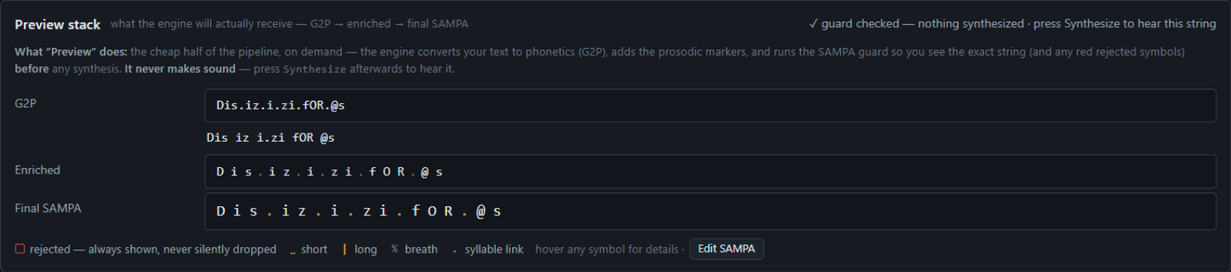
\includegraphics[width=\linewidth]{../screenshots/preview-stack.png}
\caption{The preview stack on the worked example: G2P output, the
enriched string, and the final SAMPA the engine will receive --- guard
checked, nothing synthesized yet.}
\label{fig:preview}
\end{figure}
\item \textbf{Press \key{S}} (or click \emph{Synthesize from preview}).
  A progress strip runs G2P $\rightarrow$ trajectory $\rightarrow$ VTL
  $\rightarrow$ WAV; a few seconds later the result summary appears
  (\emph{2.37\,s audio, 11 anchors, \ldots}).
\item \textbf{Press \key{Space}} to play. Watch the round \emph{polar
  display} (Figure~\ref{fig:polar}): a white head travels the trajectory,
  anchor dots light up, phonetic labels appear at their target positions,
  and the spectrogram below draws the sound with amber anchor lines.
\end{enumerate}

That is the whole loop: \emph{pick, preview, synthesize, listen, look}.

\section{The three-step pipeline}

The console is deliberately organized around three questions, printed in
the flow guide above the action bar:

\begin{enumerate}
\item \textbf{Preview --- \emph{what will the engine receive?}} Press
  \key{P}. The engine converts your text to phonetics (G2P), adds prosodic
  markers, and runs the SAMPA guard. You see the exact string --- including
  any rejected symbol in red --- \emph{before} any synthesis. This step
  never makes sound.
\item \textbf{Compile --- \emph{what is the articulation plan?}} The
  syllable compiler panel runs the engine's own anchor walk over the SAMPA
  (Section~\ref{sec:compiler}). Metric tiles, a chip per segment,
  clickable block cards. No sound either.
\item \textbf{Synthesize --- \emph{what does it sound like?}} Press
  \key{S}. The engine computes the full trajectory and renders the WAV
  through VocalTractLab. What you hear is exactly the string you inspected.
\end{enumerate}

\paragraph{The wait indicators.} Every step that contacts the engine
shows you that it is working: the Preview button relabels to
\emph{``Previewing\ldots''} (with its hourglass spinner) and a pill in
the header counts \emph{``n in flight\ldots''}. During synthesis, the progress strip
lights the current stage (G2P, trajectory, VTL, WAV, MP4) and fills a
progress bar. The polar display typically starts moving \emph{while the
WAV is still rendering} --- that is the start-early feature
(Section~\ref{sec:polar}), not a bug.

\section{Typing text vs writing SAMPA}

The \emph{Input} group has two modes. \textbf{Orthographic} is ordinary
spelling; the engine's grapheme-to-phoneme module converts it.
\textbf{Phonetic} is SAMPA, the machine-readable phonetic alphabet the
engine speaks; what you type is what the engine receives (after the guard).

Three separators matter, and the engine treats them differently:

\begin{itemize}
\item \textbf{Dot \texttt{.}} --- a syllable \emph{link}: no pause, the
  consonants around the dot form one coarticulated cluster
  (\texttt{ba.da} is one word of two syllables).
\item \textbf{Space} --- a short pause (default 200\,ms), written
  \texttt{\ovs}.
\item \textbf{Vertical bar \texttt{|}} --- a long pause (default 320\,ms),
  the phrase separator.
\item \textbf{Percent \texttt{\%}} --- a \emph{breath} pause
  (130\,ms); it also appears as a breath anchor on the display.
\item \textbf{Tilde \texttt{\~{}}} after a vowel --- nasality
  (\texttt{a\~{}} is nasalized \emph{a}, as in French \emph{banque}).
\end{itemize}

The per-language chips (EN, FR, ES, DE, IT, PT, plus two phonetic
presets and a guard demo) fill the input and trigger a preview
immediately --- the fastest way to hear each language's calibration.

\section{The red-reject guard}

The engine knows a fixed inventory of symbols ( vowels
\texttt{a e i o u y E O @ 2 6 9} plus nasals, consonants
\texttt{p b t d k g \ldots}, and the markers above). Anything else --- a
stray \texttt{c}, an IPA \emph{esh} (\texttt{S} in SAMPA), an apostrophe
--- would be \emph{silently dropped} by the engine's tokenizer. The
console refuses to let that happen quietly: such symbols are shown struck
through in red, with a count badge and a banner (Figure~\ref{fig:guard}).

\begin{figure}[htbp]
\centering
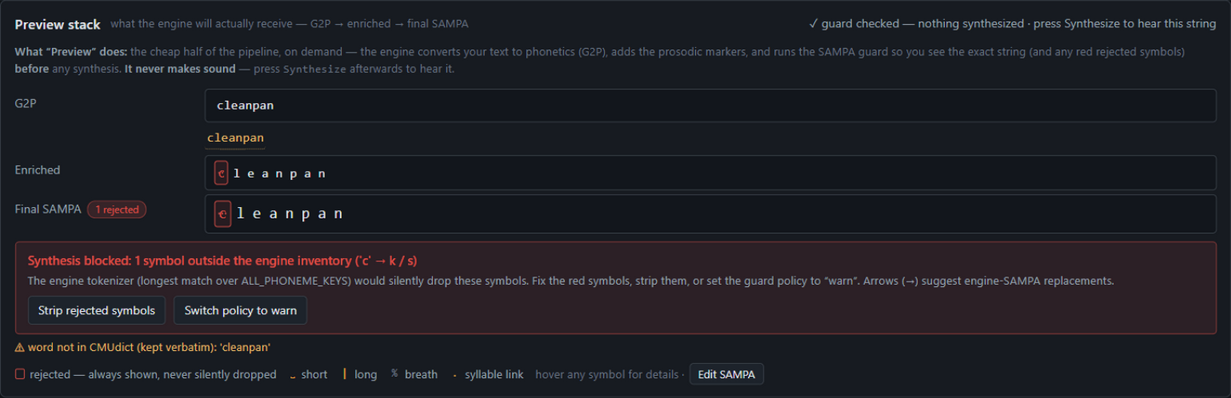
\includegraphics[width=\linewidth]{../screenshots/guard-error.png}
\caption{The guard in \texttt{error} policy on \texttt{cleanpan}: the
\texttt{c} is rejected with suggestions \texttt{k}~/~\texttt{s}, and
synthesis is blocked until you fix, strip, or downgrade the policy.}
\label{fig:guard}
\end{figure}

Three policies, in the \emph{Engine \& Guard} group:

\begin{itemize}
\item \textbf{warn} (default) --- proceed knowingly: the label changes to
  \emph{``Synthesize anyway (N dropped)''} and the engine drops the red
  symbols.
\item \textbf{error} --- blocked: no synthesis until every red symbol is
  fixed or stripped.
\item \textbf{off} --- pass-through (engine CLI semantics; know what you
  are doing).
\end{itemize}

The banner offers one-click \emph{suggestions} (\texttt{c $\rightarrow$ k
/ s}, IPA \emph{esh} $\rightarrow$ \texttt{S}, \ldots) and a
\emph{strip} action that
removes all red symbols at once. You can also hand-edit the final string:
\emph{Edit SAMPA} opens an editor on the final row; the \emph{edited}
badge reminds you the string is yours, and \key{E} synthesizes exactly
that edited string.

\section{Reading the continuous polar display}
\label{sec:polar}

\begin{figure}[htbp]
\centering
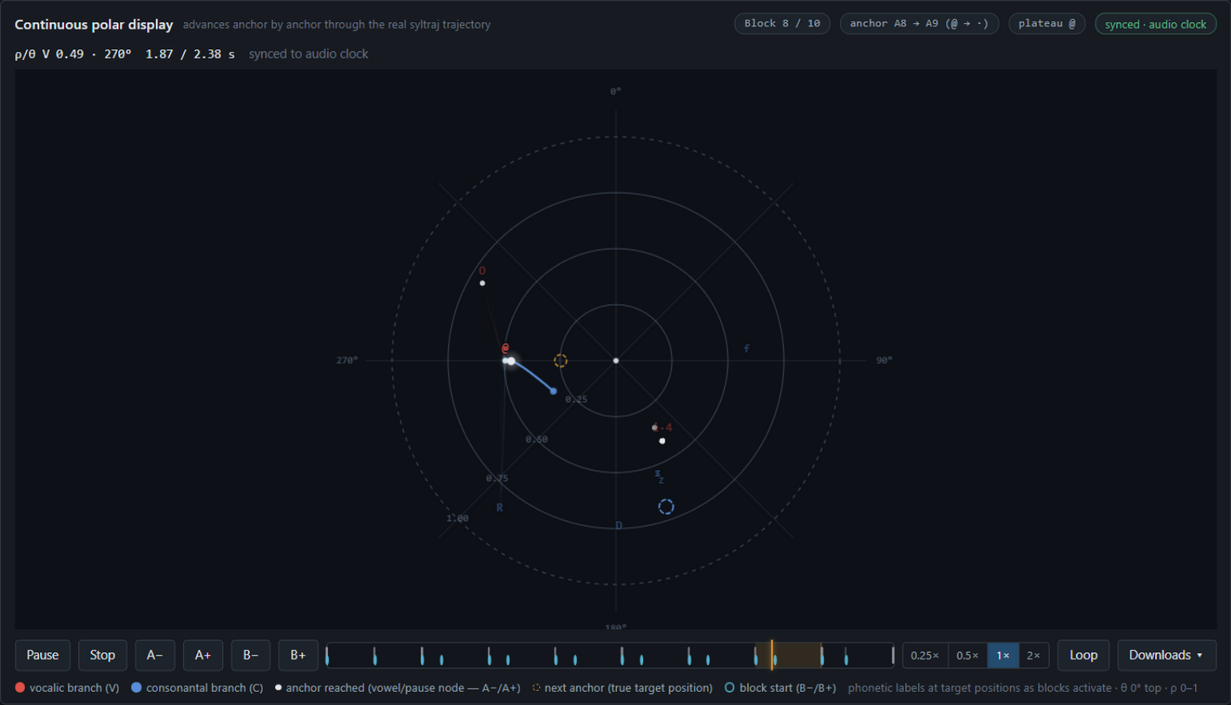
\includegraphics[width=\linewidth]{../screenshots/polar.png}
\caption{The continuous polar display mid-utterance (Block 5/10, synced
on the audio clock). Red trail: vocalic branch; blue dot and ring:
consonantal branch; small dots: anchors reached; dashed ring: next
anchor; labels appear at phoneme targets as their blocks activate.}
\label{fig:polar}
\end{figure}

The round display is the heart of the console. Angle $\theta$ runs from
the top (0\textdegree), clockwise; radius $\rho$ is normalized so the
engine's own radius range fills the disc (1.0 = the outer dashed ring).
Two branches share the disc:

\begin{itemize}
\item The \textbf{vocalic branch} (red trail) carries the vowel
  trajectory. The trail fades over roughly 300\,ms, so you see where the
  gesture \emph{came from} --- coarticulation made visible.
\item The \textbf{consonantal branch} (blue marker) carries the consonant
  closure gesture. It is only active inside consonant clusters; elsewhere
  its channels are null.
\end{itemize}

\paragraph{Labels.} Phonetic labels pop in at their target positions as
the syllabic blocks that own them activate. A count like
\textbf{``i$\cdot$4''} means \emph{four phonemes share this same target
position} --- the engine's target-sharing, printed as \texttt{key$\cdot$n}.

\paragraph{Stretches.} On the compiler cards, a segment label like
\textbf{``i\utie{}k''} reads: vowel \texttt{i} fused with the following
consonant \texttt{k}. The tie \textbf{\utie} marks consonants that follow a
vowel \emph{inside the same anchor-to-anchor stretch} --- the coda of one
syllable coarticulated with the next onset. That is exactly how the
engine groups gestures; it is not a dictionary syllable.

\paragraph{Start-early.} The trajectory (anchors, blocks, polar points)
is computed \emph{before} the audio renders. The display therefore starts
on its own clock while the WAV is still being computed --- honest, because
it is the same engine data --- and re-anchors seamlessly on the audio
clock when the sound is ready. The badge next to the block counter tells
you which clock is master: \emph{polar-only} then \emph{synced $\cdot$
audio clock}.

\section{The transport}

The bar under the polar display is a media player whose \emph{ruler} is
the anchor list:

\begin{itemize}
\item \textbf{Play / Pause} --- \key{Space} or \key{K}. \textbf{Stop}
  (back to start) --- \key{Shift+S}.
\item \textbf{\key{[} and \key{]}} --- previous / next \emph{anchor}. The
  head lands exactly on the anchor, never between.
\item \textbf{The scrub bar} --- its ticks \emph{are} the anchors; click
  a tick to snap to it. The amber band marks the current block.
  \textbf{Loop} (\key{L}) repeats the current block.
\item \textbf{Speeds} --- \key{0}--\key{3} for 0.25$\times$, 0.5$\times$,
  1$\times$, 2$\times$; applies to playback, the polar head and the
  spectrogram cursor.
\item \textbf{Downloads} (\key{D}) --- the artifacts of the current job
  (Section~\ref{sec:audio}).
\end{itemize}

Clicking a syllable-compiler card after synthesis \emph{seeks} the polar
display to exactly that segment --- the fastest way to audit one block.

\section{The syllable block compiler}
\label{sec:compiler}

\begin{figure}[htbp]
\centering
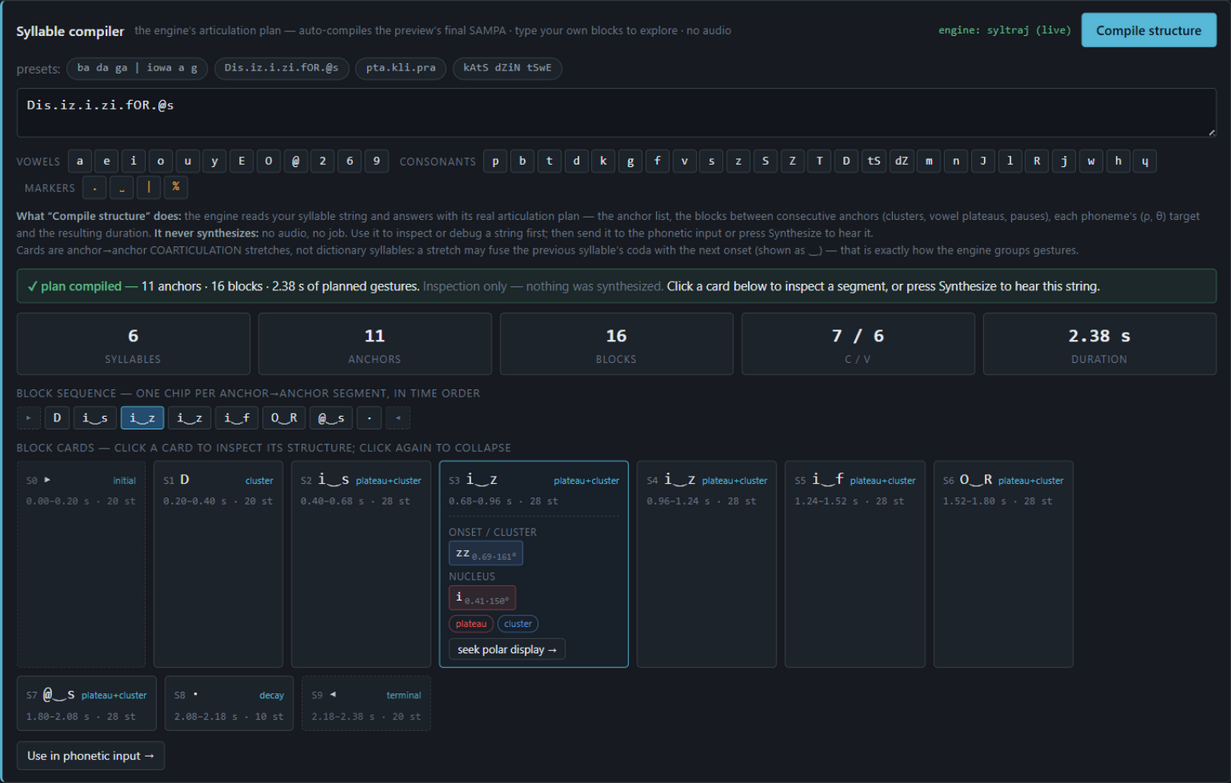
\includegraphics[width=\linewidth]{../screenshots/compiler.png}
\caption{The compiler on the worked example: metric tiles, one chip per
anchor-to-anchor segment, and clickable block cards (S3 expanded, showing
onset cluster targets in $(\rho,\theta)$ and the nucleus plateau).}
\label{fig:compiler}
\end{figure}

Press \key{C} to focus the compiler (Enter compiles). ``Compile'' means
exactly what the engine does before synthesizing --- tokenize the SAMPA,
walk the anchors, emit the block schedule --- but \emph{without} any
synthesis: it is the cheap structural half, so you can iterate freely.

The panel (Figure~\ref{fig:compiler}) shows:

\begin{itemize}
\item \textbf{Metric tiles} --- syllables, anchors, blocks, consonant and
  vowel counts, planned duration.
\item \textbf{Block sequence} --- one chip per anchor-to-anchor segment,
  in time order; the stretch labels (with the \utie{} marker) appear here.
\item \textbf{Block cards} --- click to expand: onset cluster consonants
  with their $(\rho,\theta)$ targets, the nucleus vowel plateau, block
  kinds, and time span. \emph{``Use in phonetic input $\rightarrow$''}
  pushes the compiled string to the stage (phonetic mode, previewed);
  after synthesis, clicking a card seeks the polar display to that
  segment.
\end{itemize}

The compiler auto-follows the preview: every preview's final SAMPA is
compiled automatically. Type your own blocks to explore --- the presets
(\texttt{ba da ga | iowa a g}, \texttt{pta.kli.pra}, \ldots) are one
click away. An \emph{inventory palette} of vowel, consonant and marker
chips lets you compose without typing.

\section{Timings and expressive prosody}

The \emph{Timings} group carries the four engine durations, as steppers
($\pm$10\,ms):

\begin{itemize}
\item \textbf{Tcons} --- consonantal gesture time (default 100\,ms in
  English).
\item \textbf{Tvoy} --- vocalic plateau time (default 80\,ms).
\item \textbf{tpause} / \textbf{tpause-long} --- short and long pause
  durations (200 / 320\,ms).
\end{itemize}

One engine gesture step is 10\,ms at the 100\,Hz planning rate ---
durations are rounded to steps. Each language has its own profile; a
slider that has drifted from the profile gets an amber edge, and
\emph{Reset to language profile} restores it.

The \emph{Prosody} group toggles \textbf{expressive prosody}: breathing
groups (the \texttt{\%} breath pause, 130\,ms) and an F0 contour ---
declination over each breathing group, re-attacks, pitch accents on
content words. It touches only the glottis F0 column and pause durations,
so it composes with any speaker. The \emph{Base f0} field (60--350\,Hz,
clamped) is pre-filled from the speaker registry; \emph{reset to speaker}
restores it.

\section{Audio, spectrogram, downloads and exports}
\label{sec:audio}

When a job finishes, the audio plays through the transport and the
\textbf{spectrogram} (Figure~\ref{fig:spec}) is computed locally from the
WAV. The \emph{amber vertical lines are the anchors} --- the same ticks
as the scrub bar; click anywhere on the spectrogram to seek, the polar
display follows. Buttons: \emph{f0 overlay} (draws the F0 contour on
top), \emph{Download PNG}.

\begin{figure}[htbp]
\centering
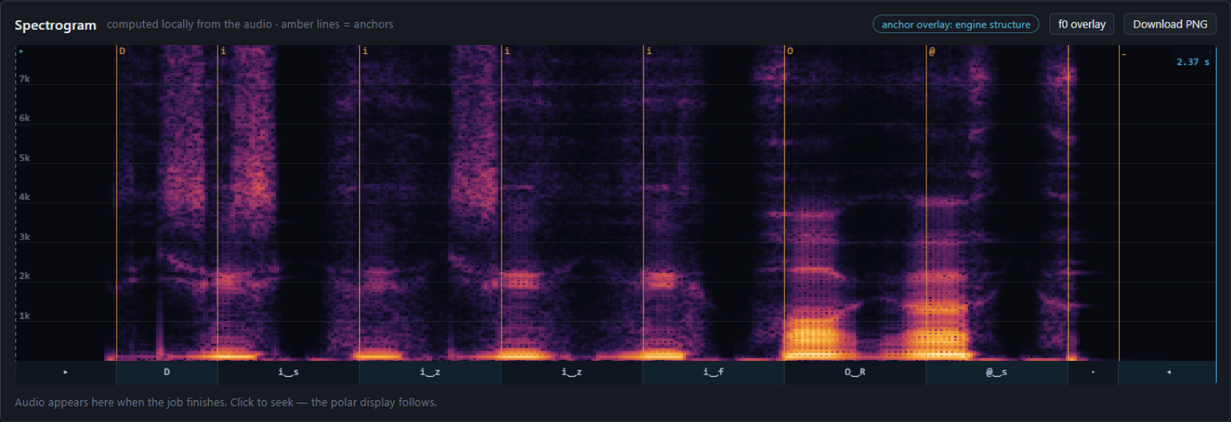
\includegraphics[width=\linewidth]{../screenshots/spectrogram.png}
\caption{Spectrogram of the worked example with the anchor overlay ---
click to seek; the polar display follows.}
\label{fig:spec}
\end{figure}

\paragraph{Downloads (\key{D}).} The WAV and the SAMPA text are
\emph{always} offered. The \textbf{Optional exports} checkbox (Display \&
Exports group) adds the TRACT file (the raw articulatory timeline) and
the polar data file. Everything lands in the console's \texttt{out/}
folder; the Display group prints the resolved absolute path so
``\texttt{out}'' is never a mystery.

\paragraph{Video.} The \emph{Output} selector can request a
\textbf{sagittal MP4} (animated mid-sagittal views) or a
\textbf{dual-panel polar MP4}. Rendering takes markedly longer than audio
and the file appears in the Downloads menu when ready; it is not shown
inline.

\section{Troubleshooting, shortcuts, FAQ}

\subsection{Troubleshooting}

\begin{longtable}{p{0.34\linewidth}p{0.62\linewidth}}
\textbf{Symptom} & \textbf{Fix} \\
\hline
Backend chip reads \emph{demo} & The bridge could not import the engine.
Start \texttt{python server.py} in the same Python environment you
installed covtl-pipeline into; check \texttt{/api/status $\rightarrow$
reason}. \\
Header shows \emph{degraded} & A registry probe failed (speaker or
lexicon). Click the backend chip for the full \texttt{/api/health}
payload; reinstall the language pack or speaker on the engine side. \\
First preview is slow & The first G2P call loads lexicons (seconds). Later
previews are cached and fast. \\
``Unverified combination'' banner & Language-pack vowels are calibrated
on the \texttt{jd3} speaker only; audio on other speakers may differ.
This is a warning, not an error. \\
No sound & Check the browser's autoplay: click \emph{Play} once (a user
gesture unlocks audio). The polar display itself runs regardless. \\
Synthesis blocked by red symbols & Fix them, use the banner's strip
action, or set the guard policy to \emph{warn} (Section~6). \\
422 on Synthesize & The guard policy is \texttt{error} and the input
still contains rejected symbols --- same fix as above. \\
Job seems stuck & Long inputs and MP4 modes take minutes. \key{Esc}
cancels. \\
Polar display freezes in a background tab & Expected: browsers throttle
background tabs; the clock catches up (watchdog), rendering resumes on
focus. \\
\end{longtable}

\subsection{Keyboard reference}

\begin{longtable}{p{0.22\linewidth}p{0.32\linewidth}p{0.2\linewidth}p{0.3\linewidth}}
\key{Space}/\key{K} & play / pause & \key{[} / \key{]} & prev / next anchor \\
\key{Shift+S} & stop (to start) & \key{L} & loop current block \\
\key{P} & preview (no sound) & \key{0}--\key{3} & speed 0.25/0.5/1/2$\times$ \\
\key{S} & synthesize current & \key{E} & synthesize edited SAMPA \\
\key{C} & focus compiler & \key{D} & downloads menu \\
\key{Esc} & cancel / stop & \key{?} & shortcut help \\
\end{longtable}

Shortcuts are plain keys, active when you are \emph{not} typing in an
editor.

\subsection{FAQ}

\textbf{Is anything sent to the internet?} No. The bridge binds
127.0.0.1 only; there is no telemetry and no cloud service.

\textbf{Why 11 anchors for ``this is easy for us'' and not 6?} The
engine's anchor list includes the utterance start, word-end anchors and
the terminal anchor --- the display follows the engine's own list, by
design.

\textbf{What exactly does Synthesize use?} The string shown in the final
SAMPA row --- the previewed one (\key{S}), your edited one (\key{E}), or
the compiler's output when you pushed it to the stage. What you see is
what you hear.

\textbf{Where are my files?} In \texttt{out/} under the console folder;
the Display \& Exports group prints the absolute path.

\textbf{Can I trust the demo mode?} For the interface and guard
semantics, yes --- they are the real code paths. The G2P, compiler and
audio are \emph{approximate simulations}, labeled as demo everywhere.

\end{document}
